\section{Experimental Evaluation}
\label{sec:experiments}
\subsection{Experimental Setup}
\subsubsection{Benchmark and Lifecycle Protocol}
Workload prediction is used as the maintenance task, following its role in proactive cloud/resource management \cite{kim2024workload,zuo2025workload,zhao2025mscnet,feng2025workloadsurvey}. Method development, decision calibration, and final evaluation use disjoint center pools; the final pool contains 30 centers, three fixed model seeds per center, and 24 chronological stages. For each target center, the initial deployed model is obtained by source pretraining followed by 50-step target warm-up adaptation on the first 800 raw observations. A disjoint 200-observation pre-maintenance interval initializes six historical verification blocks. Each stage then follows a raw-first causal split of 400 update, 240 verification, and 400 service observations; windows are formed separately within each role, giving 304/144/304 windows for $L=96,H=1$. The preceding service interval becomes the next stage's update interval only after its labels mature. The main predictor is a one-layer GRU-32; architecture/horizon generality is examined in Section~\ref{sec:sensitivity}.

\subsubsection{Method Configuration and Calibration}
Method structure is fixed on the development pool and decision parameters are calibrated on a disjoint pool before final evaluation. Each verification subset is divided into six chronological blocks, and the 12-block history is updated by FIFO truncation only after the current decision. The decision search uses $\kappa_{\mathrm{rec}},\kappa_{\mathrm{hist}}\in\{0,0.5,1.0,1.5\}$; among configurations satisfying the absolute harmful-transition and downside criteria on mixed, persistent-bias, and replay calibration settings, lifecycle MSE is minimized with a deterministic tie-break. Table~\ref{tab:configuration} reports the fixed configuration.

\begin{table}[t]
\centering
\caption{Main Experimental Configuration}
\label{tab:configuration}
\scriptsize
\begin{tabular}{lll}
\toprule
Category & Item & Setting \\
\midrule
Lifecycle & Centers / seeds / stages & 30 / 3 / 24 \\
Predictor & Architecture / input / horizon & GRU-32 / $L=96$ / $H=1$ \\
Adaptation & Optimizer / loss / updates & SGD / MSE / 50 \\
 & Learning rate / clipping & 0.01 / 1.0 \\
 & Batch / sampling / weight decay & 64 / replacement / 0 \\
Verification & Blocks per stage / history capacity & 6 / 12 blocks \\
 & $\kappa_{\mathrm{rec}},\kappa_{\mathrm{hist}}$ & $0,\ 0.5$ \\
Commitment & $\delta_{\mathrm{imp}},\delta_{\mathrm{ret}}$ & $2.8018\!\times\!10^{-5},\ 0$ \\
Risk criteria & $\rho,\epsilon$ & $0.05,\ 5.6036\!\times\!10^{-5}$ \\
Statistics & Unit / bootstrap & Center / 4000 repetitions \\
 & Model / attack / bootstrap seeds & 7311--7313 / 9417 / 2904 \\
Hardware & GPU & RTX 3060 Laptop GPU \\
\bottomrule
\end{tabular}
\end{table}

\subsubsection{Conditions, Baselines, Metrics, and Statistics}
The four benign regimes apply a deterministic scalar workload shift: stationary remains unchanged, gradual ramps from 0 to 0.8, abrupt switches to 0.8 at the stage-9 verification boundary, and recurring alternates between shifted and unshifted intervals. The mixed condition overlays telemetry corruption with nominal fraction $\alpha=0.10$ on each center's base regime. Each role segment is divided into ten temporal strata and $\lfloor n_s\alpha\rfloor$ positions per stratum are corrupted; mixed corruption cycles random noise, stage-persistent bias, bursts, and replay, while service data remain clean. Persistent-bias, replay, and additional $\alpha$ values are examined in Section~\ref{sec:severity}.

We compare RAVM-DT with Always-FT, experience replay (ER) \cite{rolnick2019replay}, elastic weight consolidation (EWC) \cite{kirkpatrick2017ewc}, Huber-loss fine-tuning (Huber-FT) \cite{huber1964robust}, ValidationCommit, and Frozen. Active methods share the 50-step adaptation budget; ER uses FIFO raw replay, EWC uses $\lambda=10$ with Fisher EMA $\gamma=0.9$, and Huber-FT uses $\delta=0.1$. ValidationCommit uses the whole-verification mean candidate--current loss difference with a calibrated threshold; its calibration triggered the retain-all fallback, yielding zero final-pool commitments. Lifecycle MSE is the primary utility metric; transition safety is measured by harmful-transition frequency and average downside, with commit rate and beneficial-commit recall characterizing adaptation. Centers are the statistical units: seeds are averaged within center and paired 95\% intervals use 4000 center-cluster bootstrap repetitions. For all methods, service data are excluded from candidate adaptation and deployment commitment.

\subsection{Overall Lifecycle Maintenance Performance}
\label{sec:overall}
\begin{figure}[t]
\centering
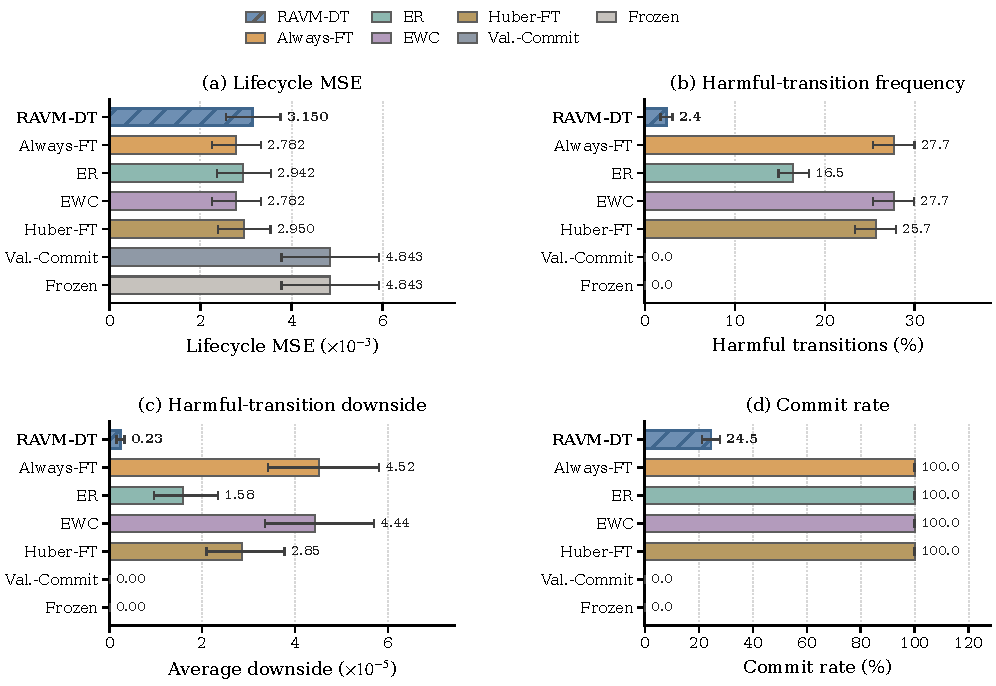
\includegraphics[width=0.80\textwidth]{fig3_overall_baseline.pdf}
\caption{Overall lifecycle performance over the five primary conditions: (a) MSE, (b) harmful-transition frequency, (c) average harmful downside, and (d) commit rate. Error bars denote 95\% center-cluster bootstrap intervals.}
\label{fig:overall}
\end{figure}

Figure~\ref{fig:overall} shows the central safety--utility--plasticity trade-off. Active always-update baselines achieve lower MSE, whereas RAVM-DT incurs about 6.8\%--13.2\% higher MSE but reduces harmful-transition frequency by about 85.5\%--91.4\% and harmful downside by 85.3\%--94.9\%. ValidationCommit makes no final-pool commitments and therefore follows Frozen; relative to this no-update reference, RAVM-DT lowers MSE by about 34.9\% while committing roughly one quarter of candidate states. Thus, its safety gain is not obtained by disabling adaptation.

\subsection{Robustness to Unreliable Monitoring Data}
\label{sec:severity}
\begin{figure}[t]
\centering
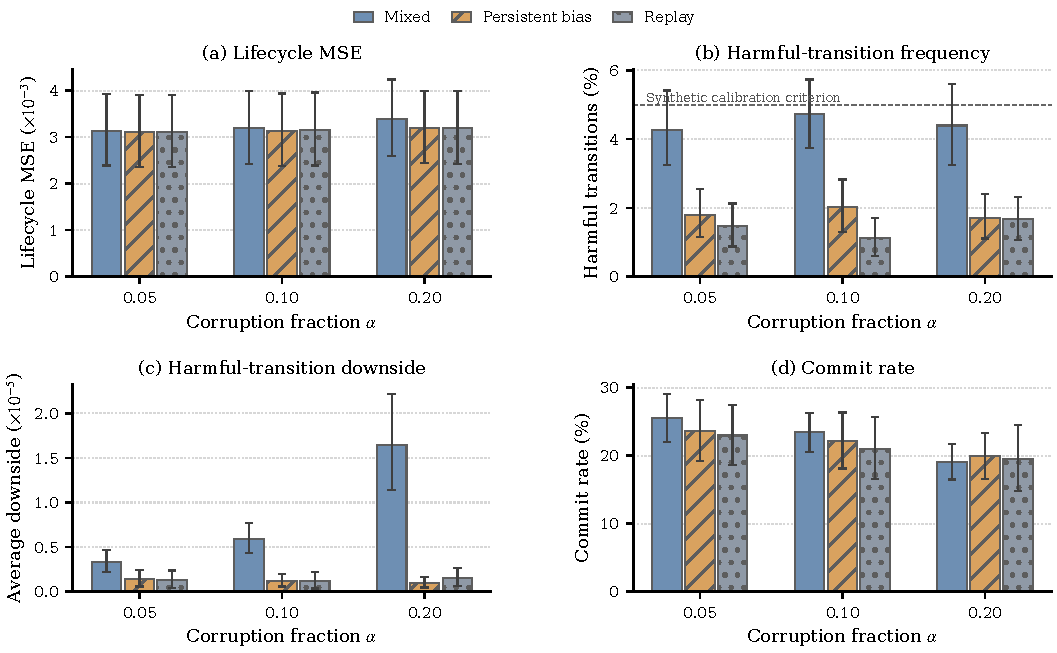
\includegraphics[width=0.74\textwidth]{fig4_corruption_severity.pdf}
\caption{Robustness across corruption severities. Mixed corruption affects update and verification data; persistent bias and replay target verification evidence. Panels report MSE, harmful-transition frequency, harmful downside, and commit rate for $\alpha\in\{0.05,0.10,0.20\}$.}
\label{fig:severity}
\end{figure}

Across the nine tested corruption--severity combinations in Fig.~\ref{fig:severity}, harmful-transition frequency remains below the 5\% synthetic-domain calibration criterion. Mixed corruption produces the clearest utility/downside deterioration as $\alpha$ increases, while commit rates decline across all three corruption types. The safety metric is not monotone in nominal corruption fraction, so the result is interpreted as robustness within the evaluated range rather than a general severity law.

\subsection{Adaptation under Benign Operating Evolution}
\label{sec:benign}
\begin{figure}[t]
\centering
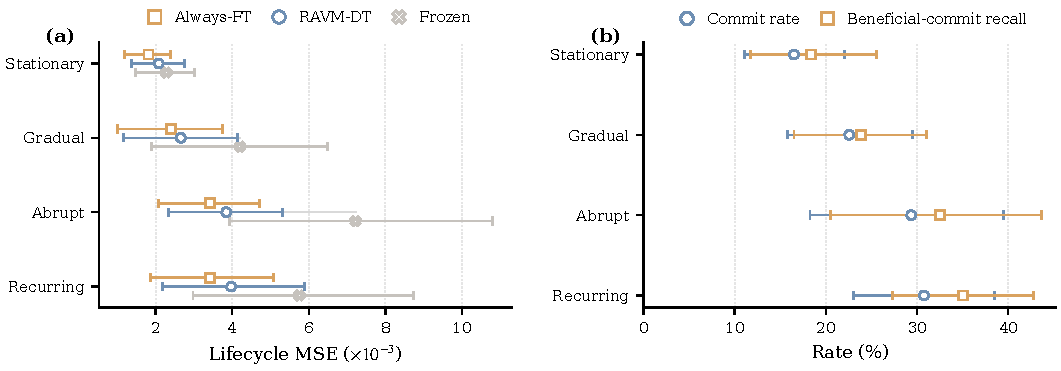
\includegraphics[width=0.70\textwidth]{fig5_benign_evolution.pdf}
\caption{Benign operating evolution: (a) lifecycle MSE for RAVM-DT, Always-FT, and Frozen; (b) RAVM-DT commit rate and beneficial-commit recall. Error bars denote 95\% center-cluster bootstrap intervals.}
\label{fig:benign}
\end{figure}

Always-FT remains the lowest-MSE reference, but RAVM-DT substantially outperforms Frozen under gradual, abrupt, and recurring drift. Its commit rate and beneficial-commit recall are higher under gradual, abrupt, and recurring drift than under stationary conditions, while harmful-transition frequency remains about 1.0\%--2.6\% across the four benign regimes. The method therefore retains selective plasticity at a measurable utility cost relative to unrestricted adaptation.

\subsection{Mechanism Analysis}
\label{sec:mechanism}
\begin{figure}[t]
\centering
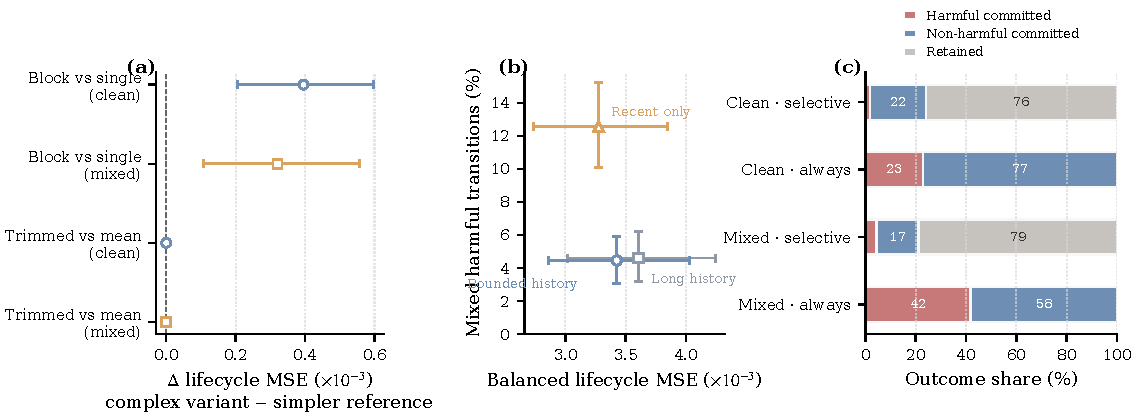
\includegraphics[width=0.78\textwidth]{fig6_mechanism_analysis.pdf}
\caption{Mechanism analysis on the development pool: (a) paired MSE effects of additional candidate-side complexity, (b) utility--risk trade-off of recent-only, long-history, and bounded-history verification, and (c) deployment outcomes for selective and always-commit variants.}
\label{fig:mechanism}
\end{figure}

Figure~\ref{fig:mechanism}(a) provides no evidence that the tested candidate-side complexity variants---blockwise construction or trimmed state-delta aggregation---improve the final maintenance outcome, supporting the simpler single-path candidate. Figure~\ref{fig:mechanism}(b) shows that recent-only verification is more plastic but reaches about 12.6\% harmful transitions under mixed corruption; adding history sharply reduces this exposure, while bounding the retained history recovers utility relative to a longer history. Finally, Fig.~\ref{fig:mechanism}(c) shows that selective commitment strongly reduces harmful replacement at the cost of retaining more candidates. Together, these results support simple candidate adaptation followed by bounded temporal verification and selective deployment control.

\subsection{Sensitivity, Generality, and Maintenance Cost}
\label{sec:sensitivity}
\begin{figure}[t]
\centering
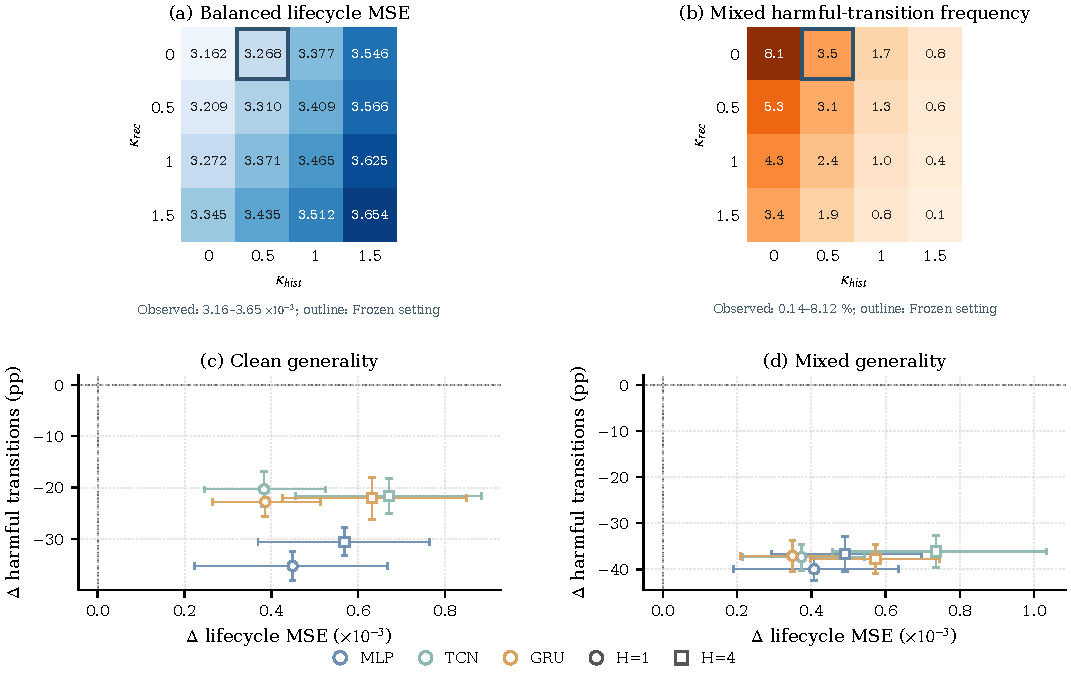
\includegraphics[width=0.72\textwidth]{fig7_sensitivity_generality.pdf}
\caption{Sensitivity and generality of RAVM-DT. Panels (a)--(b) show the predefined $\kappa_{\mathrm{rec}}\times\kappa_{\mathrm{hist}}$ grid; the outlined cell is the fixed setting $(0,0.5)$. Panels (c)--(d) show clean and mixed effects, computed as RAVM-DT minus Always-FT, across MLP, TCN, and GRU with $H\in\{1,4\}$.}
\label{fig:sensitivity}
\end{figure}

The sensitivity grid in Fig.~\ref{fig:sensitivity}(a)--(b) exposes an explicit utility--risk trade-off; the fixed setting lies on the observed frontier but is not claimed to be universally optimal. Without architecture- or horizon-specific retuning, the expected qualitative ordering is retained in all 12 tested architecture--horizon--condition cells: RAVM-DT pays a positive MSE cost relative to Always-FT while reducing harmful-transition frequency. This supports consistency across the tested settings, not architecture-invariant performance.

\begin{table}[t]
\centering
\caption{Measured Maintenance Cost in the Final Benchmark}
\label{tab:cost}
\scriptsize
\begin{tabular}{lrrr}
\toprule
Method & Runtime/stage (s) & Peak GPU (MB) & Buffer (kB) \\
\midrule
RAVM-DT & 0.185 & 55.7 & 155.5 \\
Always-FT & 0.250 & 55.6 & 0 \\
ER & 0.262 & 98.3 & 302.4 \\
EWC & 0.504 & 58.3 & 44.8 \\
Huber-FT & 0.250 & 55.6 & 0 \\
ValidationCommit & 0.252 & 67.7 & 0 \\
Frozen & 0.004 & 25.5 & 0 \\
\bottomrule
\end{tabular}
\end{table}

Table~\ref{tab:cost} shows that RAVM-DT requires about 0.185~s per maintenance stage, 55.7~MB peak GPU memory, and a 155.5~kB persistent buffer on the evaluated platform. Timing covers update construction, adaptation, verification, commitment, and maintenance bookkeeping, but excludes subsequent service evaluation and file I/O. Its runtime is of the same order as the adaptive baselines; these measurements characterize the implementation rather than a general latency guarantee.

\subsection{External Production-Trace Evaluation}
\label{sec:external}
\begin{figure}[t]
\centering
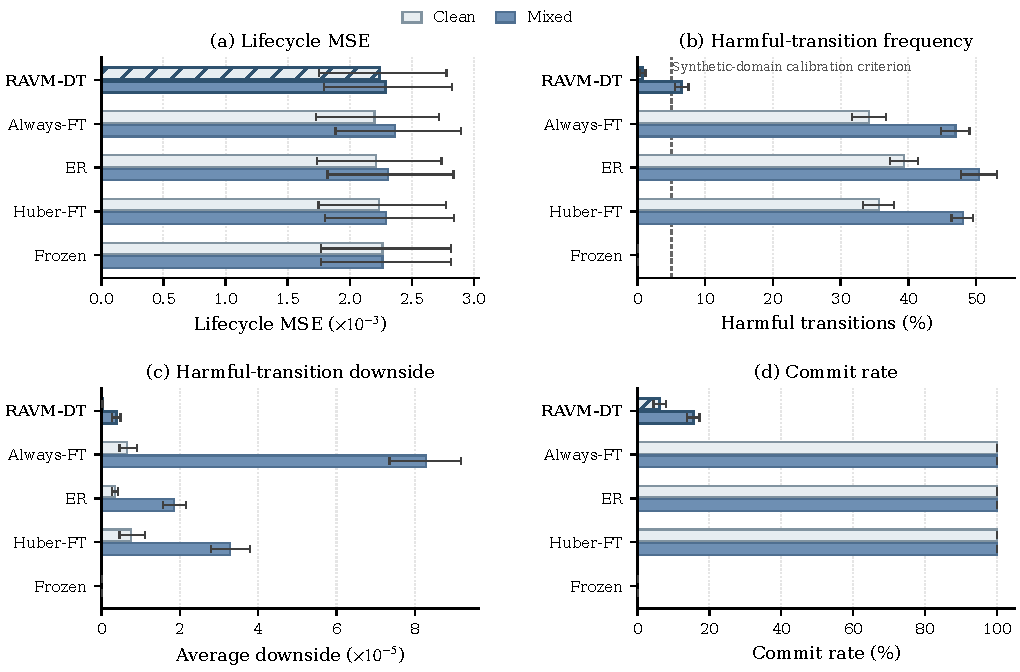
\includegraphics[width=0.68\textwidth]{fig8_alibaba_external.pdf}
\caption{External Alibaba-trace evaluation under clean and mixed corruption. Panels report (a) lifecycle MSE, (b) harmful-transition frequency, (c) harmful downside, and (d) commit rate. The 5\% line in (b) is the synthetic-domain calibration criterion.}
\label{fig:external}
\end{figure}

We finally evaluate the fixed configuration on the reconstructed 40-machine Alibaba Cluster Trace split \cite{alibaba2018trace}, without target-domain recalibration. For each selected machine, the first 17,000 valid timestamp-sorted observations are retained without interpolation; seven telemetry values are represented with value/mask channels and processed by the same causal lifecycle protocol. Under clean workloads, RAVM-DT is close to the active baselines in MSE while showing much lower harmful-transition exposure. Under mixed corruption, it remains selectively active and strongly reduces harmful transitions/downside relative to active baselines, but its harmful-transition frequency reaches 6.49\%, above the 5\% synthetic-domain calibration criterion, and its MSE is slightly higher than Frozen. The result therefore supports qualitative transfer of selective state-transition control, while showing that the exact risk operating point can be domain dependent.
